% !TEX program = xelatex
\documentclass[11pt]{article}

% ---------- Packages ----------
\usepackage[margin=1in]{geometry}
\usepackage{graphicx}
\usepackage{booktabs}
\usepackage{caption}
\usepackage{subcaption}
\usepackage{amsmath}
\usepackage{amssymb}
\usepackage{xcolor}
\usepackage{titlesec}
\usepackage{fancyhdr}
\usepackage{setspace}
\usepackage{parskip}

% بسته natbib برای دستورهای cite اضافه شد
\usepackage{natbib}

\usepackage{hyperref}
\usepackage{enumitem}
\usepackage{array}
\usepackage{tabularx}
\usepackage{longtable}

% تنظیم مسیر تصاویر
\graphicspath{{./}{../figures/}}

% تعریف رنگ‌ها
\definecolor{econred}{RGB}{194,26,30}
\definecolor{econgray}{RGB}{80,80,80}

% تنظیم استایل بخش‌ها
\titleformat{\section}{\normalfont\Large\bfseries\color{econred}}{\thesection}{1em}{}
\titleformat{\subsection}{\normalfont\large\bfseries\color{black}}{\thesubsection}{1em}{}
\titlespacing*{\section}{0pt}{1.5em}{0.8em}

% تنظیم سربرگ و پابرگ
\pagestyle{fancy}
\fancyhf{}
\fancyhead[R]{\small\itshape پروژه اقتصاد کلان}
\fancyhead[L]{\small\itshape بررسی مجدد شوک یارانه انرژی ایران}
\fancyfoot[C]{\thepage}
\renewcommand{\headrulewidth}{0.4pt}

% تنظیمات لینک‌ها
\hypersetup{
    colorlinks=true,
    linkcolor=econred,
    citecolor=econred,
    urlcolor=econgray
}

\setstretch{1.06}

% دستور برای نمایش لایتینگ لغات/متغیرهای انگلیسی از چپ به راست
\newcommand{\coef}[1]{\texttt{\lr{#1}}}

% تعریف ستون‌های سفارشی tabularx
\newcolumntype{Y}{>{\raggedleft\arraybackslash}X}
\newcolumntype{Z}{>{\centering\arraybackslash}X}

% xepersian باید آخرین پکیجی باشد که فراخوانی می‌شود
\usepackage{xepersian}
\IfFontExistsTF{XB Niloofar}{\settextfont{XB Niloofar}}{\settextfont{Noto Naskh Arabic}}

\title{
    \begin{LTR}
    \IfFileExists{sharif-logo-png-transparent.png}{\includegraphics[width=0.25\textwidth]{sharif-logo-png-transparent.png}}{}
    \end{LTR}
    \vspace{0.8cm}
    \vspace{-2em}
    {\color{econgray}\rule{\linewidth}{1pt}}\\[0.3em]
    {\Huge \bfseries پروژه اقتصاد کلان}\\[0.4em]
    {\Large \itshape فناوری صنعتی، شدت سرمایه‌گذاری و مواجهه با اصلاح قیمت انرژی:\\
شواهدی از صنایع تولیدی ایران}\\[0.3em]
    {\color{econgray}\rule{\linewidth}{1pt}}
}

\author{علیرضا فرجی | پردیس رحیمی نصر | آمیار سی و سه مرده \\[0.5em] 
\normalsize استاد درس: \textbf{دکتر بخشیانی}
}
\date{\small\today}

\begin{document}
\maketitle

\begin{abstract}
این مقاله آثار اصلاح یارانه‌های انرژی ایران در آذر ۱۳۸۹ بر عملکرد بخش تولید را دوباره بررسی می‌کند. ابتدا برآوردهای اثرات ثابت (\lr{fixed effects}) \citet{zarepour2023} را بازتولید می‌کنیم؛ سپس مقایسه دودویی میان گروه تیمار و کنترل را در کنار نگه می‌داریم و یک سنجه پیوسته از مواجهه مستقیم پیش از اصلاح و یک جانشین برای مواجهه غیرمستقیم از مسیر نهاده‌های واسطه‌ای می‌سازیم. پنل مورد استفاده شامل ۵٬۶۳۶ مشاهده مربوط به ۱٬۳۳۶ گروه صنعت چهاررقمی--استان در فاصله سال‌های ۲۰۰۹ تا ۲۰۱۳ است. بازتولید دودویی نشان می‌دهد که تولید، ارزش افزوده و مازاد عملیاتی در گروه‌های حساس به انرژی، نسبت به گروه‌های کمتر حساس، به‌ترتیب ۳٫۳۵، ۷٫۳۰ و ۹٫۱۲ درصد کاهش یافته است؛ این ضرایب یک اثر نسبی را اندازه می‌گیرند، نه اثر اصلاح در مقایسه با نبود سیاست. در الگوی دوز پیوسته، افزایش یک انحراف معیار در مواجهه مستقیم با ۰٫۰۵۱ واحد لگاریتمی تولید بیشتر پس از اصلاح همراه است، اما این ضریب اثر علّی را شناسایی نمی‌کند و معناداری آن به روش استنباط حساس است: مقدار $p$ از ۰٫۰۱۵ با خوشه‌بندی واحد به ۰٫۱۹۴ با خوشه‌بندی صنعت و ۰٫۲۲۲ با خوشه‌بندی دوطرفه می‌رسد. فناوری صنعتی و شدت سرمایه‌گذاری با تفاوت در ظرفیت تعدیل مرتبط‌اند، اما هر دو سنجه در سطح صنعت--استان تعریف شده‌اند و برای شناسایی اثر علّی فناوری یا موجودی سرمایه مناسب نیستند. انتقال مستقیم و غیرمستقیم شوک، حاشیه‌های تعدیل، عدم توازن نمونه، و محدودیت ناشی از تنها دو سال پیش از اصلاح نیز در ادامه مستند شده‌اند.


\end{abstract}
\newpage
\section{مقدمه}

یارانه‌های انرژی قیمت‌های نسبی را در سراسر شبکه تولید تغییر می‌دهند. حذف آن‌ها می‌تواند پیامدهای مالی و زیست‌محیطی را بهبود دهد، اما اصلاح ناگهانی قیمت‌ها ممکن است تولید را کاهش دهد، سود را فشرده سازد و بخشی از موجودی سرمایه موجود را به‌طور موقت غیراقتصادی کند. اصلاح آذر ۱۳۸۹ ایران از این جهت موردی آموزنده است که قیمت چند حامل انرژی به‌صورت ناگهانی افزایش یافت و این تغییر کل اقتصاد را دربر گرفت. بنگاه‌های تولیدی هزینه بیشتری برای سوخت و برق پرداخت کردند. هم‌زمان، قیمت مواد اولیه‌ای که انرژی در آن‌ها نهفته بود افزایش یافت و تقاضای خانوار تضعیف شد. بنابراین، این رویداد واکنش بنگاه‌ها را به پرسش‌های اقتصاد کلان درباره اعوجاج‌ها، بهره‌وری، سرمایه‌گذاری و انتشار شوک پیوند می‌دهد.

نقطه آغاز تحلیل ما مطالعه \citet{zarepour2023} است که یک مقایسه شبه‌آزمایشی (\lr{quasi-experimental}) میان گروه‌های تولیدی حساس به انرژی و گروه‌های کمتر حساس ایجاد می‌کنند. برآوردهای تفاضل در تفاضل (\lr{Difference-in-Differences, DID}) ترجیحی آنان از کاهش‌های اقتصادی معنادار در تولید، ارزش افزوده و مازاد عملیاتی حکایت دارد.

کار خود را با یک مرحله اعتبارسنجی بازتولید آغاز می‌کنیم؛ پیش از تفسیر هرگونه بسط، پیاده‌سازی پایتون باید ضرایب مرجع و خطاهای استاندارد خوشه‌بندی‌شده را بازتولید کند. بعد از آن سراغ پرسش دیگری می‌رویم: به‌جای قرار دادن هر واحد در یکی از دو گروه مواجهه، میانگین سهم هزینه انرژی آن در سال‌های ۲۰۰۹ و ۲۰۱۰ را به‌عنوان دوز پیوسته تیمار به کار می‌بریم و سهم نهاده‌های واسطه‌ای را هم برای تقریب مواجهه غیرمستقیم می‌سازیم. هر دو دوز به‌طور هم‌زمان برآورد می‌شوند، ضرایب پویا و شیوه‌های مختلف خوشه‌بندی مقایسه می‌شوند، و تعدیل در مصرف انرژی، تشکیل سرمایه، جبران خدمات کارکنان، مواد اولیه، تعداد بنگاه‌ها و خدمات تولیدی بررسی می‌شود.

تمرکز محتوایی مقاله بر ناهمگنی واحدهای صنعت--استان و ظرفیت تعدیل آن‌هاست. یک شوک مشترک قیمت انرژی واکنشی یکسان ایجاد نمی‌کند، چون بنگاه‌ها با فناوری‌ها و موقعیت‌های سرمایه‌ای متفاوت وارد دوره اصلاح می‌شوند. این نکته با سه رشته ادبیات پیوند دارد: بنگاه‌های ناهمگن باعث می‌شوند اعوجاج‌های سیاستی اثر متفاوتی داشته باشند \cite{restuccia2008,hsieh2009}، پذیرش فناوری معمولاً با موانعی روبه‌رو می‌شود \cite{parente1994}، و تخصیص نادرست سرمایه (\lr{misallocation}) خودش بهره‌وری را تغییر می‌دهد \cite{david2019}. در عمل، صنایعی که در طبقات فناوری بالاتر قرار می‌گیرند ممکن است مجموعه جانشینی گسترده‌تری داشته باشند و واحدهایی با شدت سرمایه‌گذاری بالاتر ممکن است ظرفیت تعدیل متفاوتی داشته باشند -- هرچند تجهیزات تخصصی می‌توانند برعکس عمل کنند و تولید را به یک روش انرژی‌بر گره بزنند.

بازتولید دودویی یک اثر نسبی منفی را تأیید می‌کند، اما برآورد تولید در الگوی ترجیحی دوز پیوسته مثبت است -- و این مثبت بودن به شیوه خوشه‌بندی حساس است. باید توجه داشت این ضریب عملکرد متفاوت را در نمونه‌ای با کنترل‌های فراوان اندازه می‌گیرد، نه اثر کل اصلاح را. نتیجه اقتصادی اصلی مقاله از برآوردهای ناهمگنی می‌آید: گروه‌های کم‌فناوری زیان بیشتری نشان می‌دهند، و اثر منفی روی گروه‌های دارای شدت سرمایه‌گذاری بالا کوچک‌تر از برآورد قبل و بعد در کل نمونه است. تشکیل سرمایه هم هیچ واکنش کوتاه‌مدت قابل تشخیصی نسبت به دوز نشان نمی‌دهد.

سهم اصلی ما قرار دادن طبقه‌بندی فناوری صنعتی و شدت سرمایه‌گذاری در مرکز تفسیر تجربی است. مطالعه مرجع را بازتولید می‌کنیم، تقسیم‌بندی خشن مواجهه را با طرح دوز--پاسخ جایگزین می‌سازیم و مواجهه مستقیم و غیرمستقیم را جداگانه بررسی می‌کنیم. سپس فناوری صنعتی و شدت سرمایه‌گذاری توضیح می‌دهند که چرا مواجهه‌های ظاهراً مشابه الزاماً به واکنش یکسان منجر نمی‌شوند. \citet{zarepour2023} برآوردهای زیرگروهی مرتبطی ارائه می‌کنند، اما آن برآوردها نقش آزمون‌های تکمیلی ناهمگنی را دارند. در این مقاله، طبقه‌بندی فناوری صنعتی و شدت سرمایه‌گذاری پرسش پژوهش، ارزیابی توازن و تفسیر حاشیه‌های تعدیل را سازمان می‌دهند.

\section{اصلاح یارانه انرژی و صنایع تولیدی ایران}

پیش از اصلاح، ایران یارانه‌های بزرگی برای بنزین، برق، گاز طبیعی و سایر حامل‌های انرژی پرداخت می‌کرد. در آذر ۱۳۸۹ قیمت‌های اداری به‌شدت افزایش یافتند. مطالعه مرجع از رشد تقریباً شش‌برابری قیمت نفت سفید، نزدیک به چهاربرابر شدن قیمت گاز طبیعی و تقریباً دوبرابر شدن قیمت بنزین و برق گزارش می‌دهد. بخش تولید از این سیاست مستثنا نبود. از آنجا که سیاست در سراسر اقتصاد اجرا شد، هیچ بخش تولیدی واقعاً تیمارنشده‌ای وجود ندارد؛ گروه کنترل تجربی تنها می‌تواند شامل واحدهایی باشد که حساسیت کمتری به شوک داشتند.

اصلاح از سه مسیر بر عملکرد اثر می‌گذارد. مسیر مستقیم از خرید سوخت و برق خود بنگاه‌ها عبور می‌کند. اگر قیمت محصولات نتواند بی‌درنگ تعدیل شود، هزینه نهایی بالا می‌رود و تولید و مازاد عملیاتی کاهش می‌یابد. مسیر غیرمستقیم از شبکه‌های تولید می‌گذرد. عرضه‌کنندگان بالادستی انرژی‌بر قیمت فولاد، سیمان، مواد شیمیایی، حمل‌ونقل، بسته‌بندی و سایر نهاده‌های واسطه‌ای را افزایش می‌دهند. ازاین‌رو، یک بنگاه پایین‌دستی با صورتحساب انرژی کوچک نیز می‌تواند با شوک مؤثری بزرگ روبه‌رو شود. مسیر تقاضا هنگامی شکل می‌گیرد که افزایش مخارج انرژی خانوار و تورم عمومی، قدرت خرید واقعی را کاهش دهد. انقباض حاصل به‌ویژه برای تولیدکنندگان کالاهای نهایی مهم است. این مسیر در این پروژه به‌عنوان سازوکار زمینه‌ای مطرح می‌شود و مستقیماً شناسایی نمی‌شود.

\section{فناوری صنعتی، شدت سرمایه‌گذاری و واکنش واحد صنعت--استان}

فناوری صنعتی و شدت سرمایه‌گذاری می‌توانند هر سه مسیر را شکل دهند، اما داده‌های ما ظرفیت تعدیل را در سطح واحد صنعت--استان اندازه‌گیری می‌کنند. فناوری کشش جانشینی امکان‌پذیر میان انرژی، نیروی کار، مواد اولیه و سرمایه را تغییر می‌دهد. پایش انرژی، ماشین‌آلات جدید و بازطراحی فرایند می‌توانند انرژی مورد نیاز برای تولید هر واحد محصول را کاهش دهند. این سازوکار، اصلاح را به موانع پذیرش فناوری مورد تأکید \citet{parente1994} و نیز به ادبیات بازتخصیص و بهره‌وری، از جمله \citet{olley1996} و \citet{hsieh2009}، مرتبط می‌کند. شدت سرمایه‌گذاری نقشی دوگانه در تفسیر دارد. سرمایه‌گذاری و دسترسی به منابع مالی ممکن است امکان اصلاح تجهیزات را بیشتر کند، اما نسبت مشاهده‌شده تشکیل سرمایه ثابت به تولید، موجودی سرمایه انباشته یا ظرفیت مالی را به‌طور مستقیم اندازه‌گیری نمی‌کند. بااین‌حال، ماشین‌آلات تخصصی ممکن است مکمل انرژی باشند و جایگزینی آن‌ها هزینه زیادی داشته باشد؛ بنابراین شدت سرمایه‌گذاری بالاتر لزوماً به معنای انعطاف‌پذیری بیشتر نیست. ادبیات سرمایه‌گذاری، تعدیل کند را در شرایط جریان نقدی ضعیف یا نااطمینانی بالا پیش‌بینی می‌کند.
\text{\citep{gilchrist1995,bloom2009}}
تحریم‌های بعدی و نوسان‌های اقتصاد کلان ایران این رفتار انتظار و مشاهده را تقویت کردند.

تعدیل تولیدکنندگان بزرگ یا مرتبط در سراسر اقتصاد انتشار می‌یابد و با دیدگاه دانه‌ای (\lr{granular}) \citet{gabaix2011} سازگار است. این موضوع اصلاح انرژی را به تخصیص نادرست، سرمایه‌گذاری و انتقال شوک در منابع ارائه‌شده پیوند می‌دهد.

\section{داده‌ها و اندازه‌گیری}

داده‌ها یک پنل سالانه نامتوازن از واحدهای تولیدی ایران است که در سطح گروه‌های صنعت چهاررقمی \lr{ISIC} در استان تجمیع شده‌اند. یک واحد زمانی وارد نمونه می‌شود که دست‌کم دو بنگاه دارای ده کارکن یا بیشتر در همان صنعت و استان فعالیت کنند. فایل شامل ۵٬۶۳۶ مشاهده واحد--سال، ۱٬۳۳۶ گروه متمایز و سال‌های ۲۰۰۹ تا ۲۰۱۳ است. تعداد مشاهدات پیش از اصلاح ۲٬۲۶۷ و پس از اصلاح ۳٬۳۶۹ است. تولید، ارزش افزوده تولیدی و مازاد عملیاتی به‌صورت لگاریتمی بیان شده‌اند و متغیرهای وابسته اصلی را تشکیل می‌دهند. کنترل‌های نهاده‌ای شامل مواد اولیه، ابزارهای بی‌دوام، بسته‌بندی، انرژی، آب، خدمات تولیدی، جبران خدمات کارکنان، تشکیل سرمایه و تعداد بنگاه‌هاست. صادرات نفت نیز به‌عنوان جانشینی برای تحریم‌ها و فشار مشترک اقتصاد کلان به کار می‌رود.

پنل در اطراف تاریخ سیاست کامل نیست. از میان ۱٬۳۳۶ واحد، ۱٬۰۵۴ واحد در هر دو سال ۲۰۰۹ و ۲۰۱۰ حضور دارند، ۱۵۹ واحد تنها در یکی از این دو سال مشاهده می‌شوند و ۱۲۳ واحد هیچ مشاهده پیش از اصلاح ندارند. ساخت دوز پیش از اصلاح، ۱٬۲۱۳ واحد و ۵٬۴۲۶ مشاهده باقی می‌گذارد. دوز مستقیم به‌صورت زیر تعریف می‌شود:
\begin{equation}
D_i=\frac{1}{n_i^{pre}}\sum_{t\in\{2009,2010\}}
\exp\!\left(\log E_{it}-\log Y_{it}\right),
\end{equation}
که در آن $E$ مخارج انرژی و $Y$ تولید است. در دوز غیرمستقیم، انرژی با مجموع سهم مخارج مواد اولیه، بسته‌بندی و ابزارهای بی‌دوام جایگزین می‌شود. هر دو سنجه ابتدا در صدک‌های اول و نودونهم وینزور (\lr{winsorize}) -- یعنی مقادیر پرت به این دو صدک محدود -- و سپس استاندارد می‌شوند. میانگین بدون وزن سهم انرژی پیش از اصلاح تقریباً ۲٫۰ درصد است و سهم کل موزون‌شده با ارزش ۱٫۳ درصد. سنجه غیرمستقیم را باید جانشینی برای وابستگی به نهاده‌های واسطه‌ای دید، نه مشاهده مستقیم انرژی نهفته در محصولات عرضه‌کنندگان.

فناوری از طبقه‌بندی صنعتی \lr{OECD} پیروی می‌کند. رده‌های ۱ و ۲ به‌عنوان فناوری پایین یا متوسط رو به پایین و رده‌های ۳ و ۴ به‌عنوان فناوری متوسط رو به بالا یا بالا کدگذاری می‌شوند. شدت سرمایه‌گذاری با نسبت تشکیل سرمایه ثابت به تولید تقریب زده می‌شود و در کد بازتولید، مقدار ۰٫۰۶ آستانه شدت سرمایه‌گذاری بالا است. این سنجه‌ها در سطح گروه تعریف شده‌اند: آن‌ها یک سلول صنعت--استان را توصیف می‌کنند، نه فناوری اختصاصی، موجودی سرمایه یا ترازنامه یک بنگاه منفرد را.

\begin{table}[htbp]
\centering
\caption{ساختار نمونه و توازن تیمار}
\label{tab:sample}
\small
\begin{tabularx}{\textwidth}{Yrrrr}
\toprule
گروه & شناسه‌های تیمار & شناسه‌های کنترل & مشاهدات تیمار & مشاهدات کنترل \\
\midrule
تمام گروه‌های فناوری & ۱٬۱۷۳ & ۱۶۳ & ۴٬۹۶۸ & ۶۶۸ \\
فناوری پایین و متوسط رو به پایین & ۹۰۵ & ۵۹ & ۳٬۸۶۱ & ۲۱۷ \\
فناوری متوسط رو به بالا و بالا & ۲۶۸ & ۱۰۴ & ۱٬۱۰۷ & ۴۵۱ \\
\bottomrule
\end{tabularx}
\begin{flushright}\footnotesize
توضیحات: «تیمار» به صنایع حساس به انرژی در طرح دودویی اشاره دارد. تعداد واحدها بر پایه طبقه‌بندی‌های ثابت در طول زمانِ تیمار و فناوری برای ۱٬۳۳۶ گروه منحصربه‌فرد صنعت--استان محاسبه شده است.
\end{flushright}
\end{table}

\section{بررسی روندها پیش از اجرای رگرسیون‌ها}

شکل~\ref{fig:trends} میانگین‌های خام سال به سالِ لگاریتم تولید، ارزش افزوده و مازاد عملیاتی را برای گروه‌های تیمار و کنترل ترسیم می‌کند؛ خط‌چین پایان سال ۲۰۱۰ را نشان می‌دهد. الگو ساده است: هر دو گروه در طول سال ۲۰۱۱ افت می‌کنند و بعد تا حدی بهبود می‌یابند، یعنی همان افت و بازگشت نسبی در هر دو سری دیده می‌شود -- دقیقاً چیزی که وقتی یک شوک مشترک در کنار سایر نیروهای کلان اقتصادی عمل می‌کند، انتظارش را داریم.

کانال هزینه مستقیم را شکل~\ref{fig:energy} روشن‌تر نشان می‌دهد: میانگین لگاریتم هزینه سوخت، برق و کل انرژی در تمام گروه‌های صنعت--استان در سال ۲۰۱۱ (نخستین سال کامل پس از اصلاحات) به‌طور قابل‌توجهی بالا می‌رود و در ۲۰۱۲--۲۰۱۳ کمی عقب می‌نشیند -- احتمالاً به دلیل تعدیل ترکیب نهاده‌ها یا افت تولید. باید تأکید کرد که هیچ‌یک از این دو شکل به‌تنهایی یک اثر علی (\lr{causal effect}) را شناسایی نمی‌کند؛ این کار به عهده رگرسیون‌های بخش بعد است. آنچه این دو شکل نشان می‌دهند صرفاً این است که ردپای اصلاحات، پیش از هرگونه انتخاب مدلی، در داده‌ها قابل مشاهده است.

\begin{figure}[htbp]
\centering
\IfFileExists{trend_by_group.png}{%
    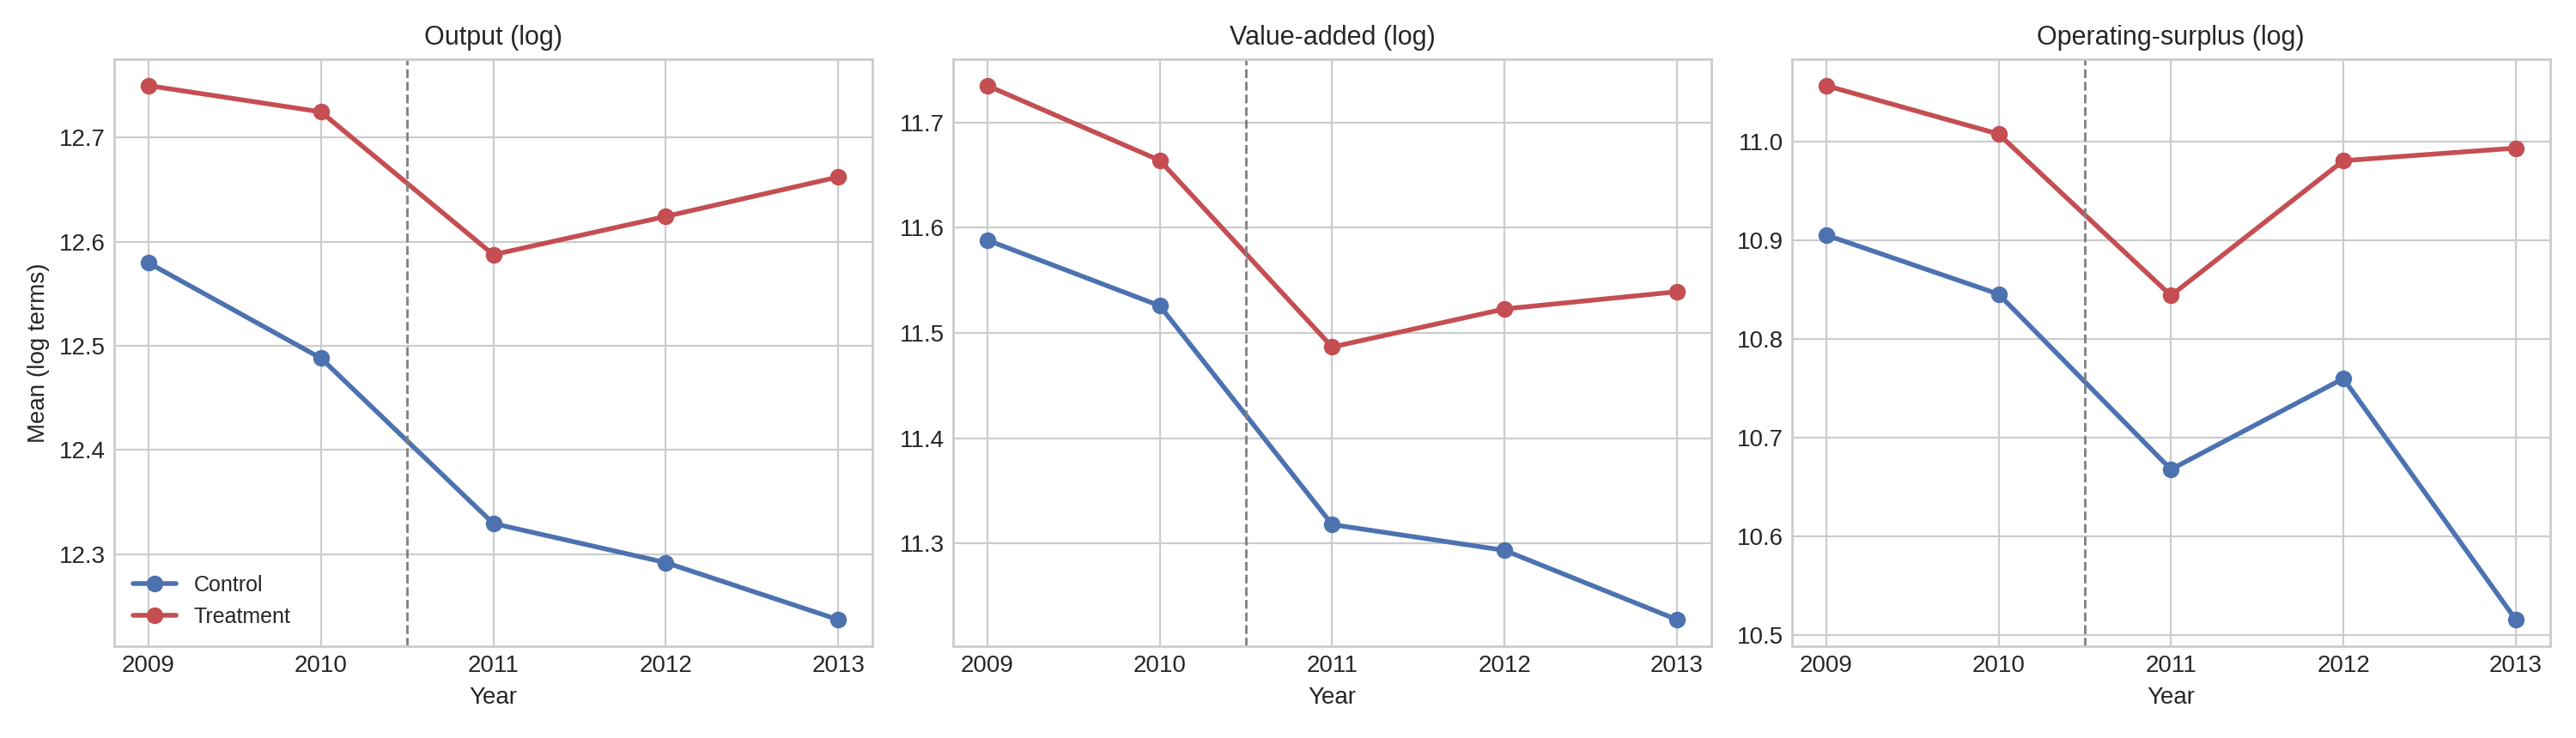
\includegraphics[width=\textwidth]{trend_by_group.png}%
}{%
    \fbox{\parbox[c][5cm][c]{0.92\textwidth}{\centering محل قرارگیری نمودار روند گروه‌های تیمار و کنترل}}%
}
\caption{میانگین لگاریتم تولید، ارزش افزوده و مازاد عملیاتی بر حسب سال، برای گروه‌های تیمار (حساس به انرژی) و کنترل (کم‌تر حساس به انرژی). خط‌چین نشان‌دهنده اصلاحات دسامبر ۲۰۱۰ است.}
\label{fig:trends}
\end{figure}

\begin{figure}[htbp]
\centering
\IfFileExists{energy_input_trend.png}{%
    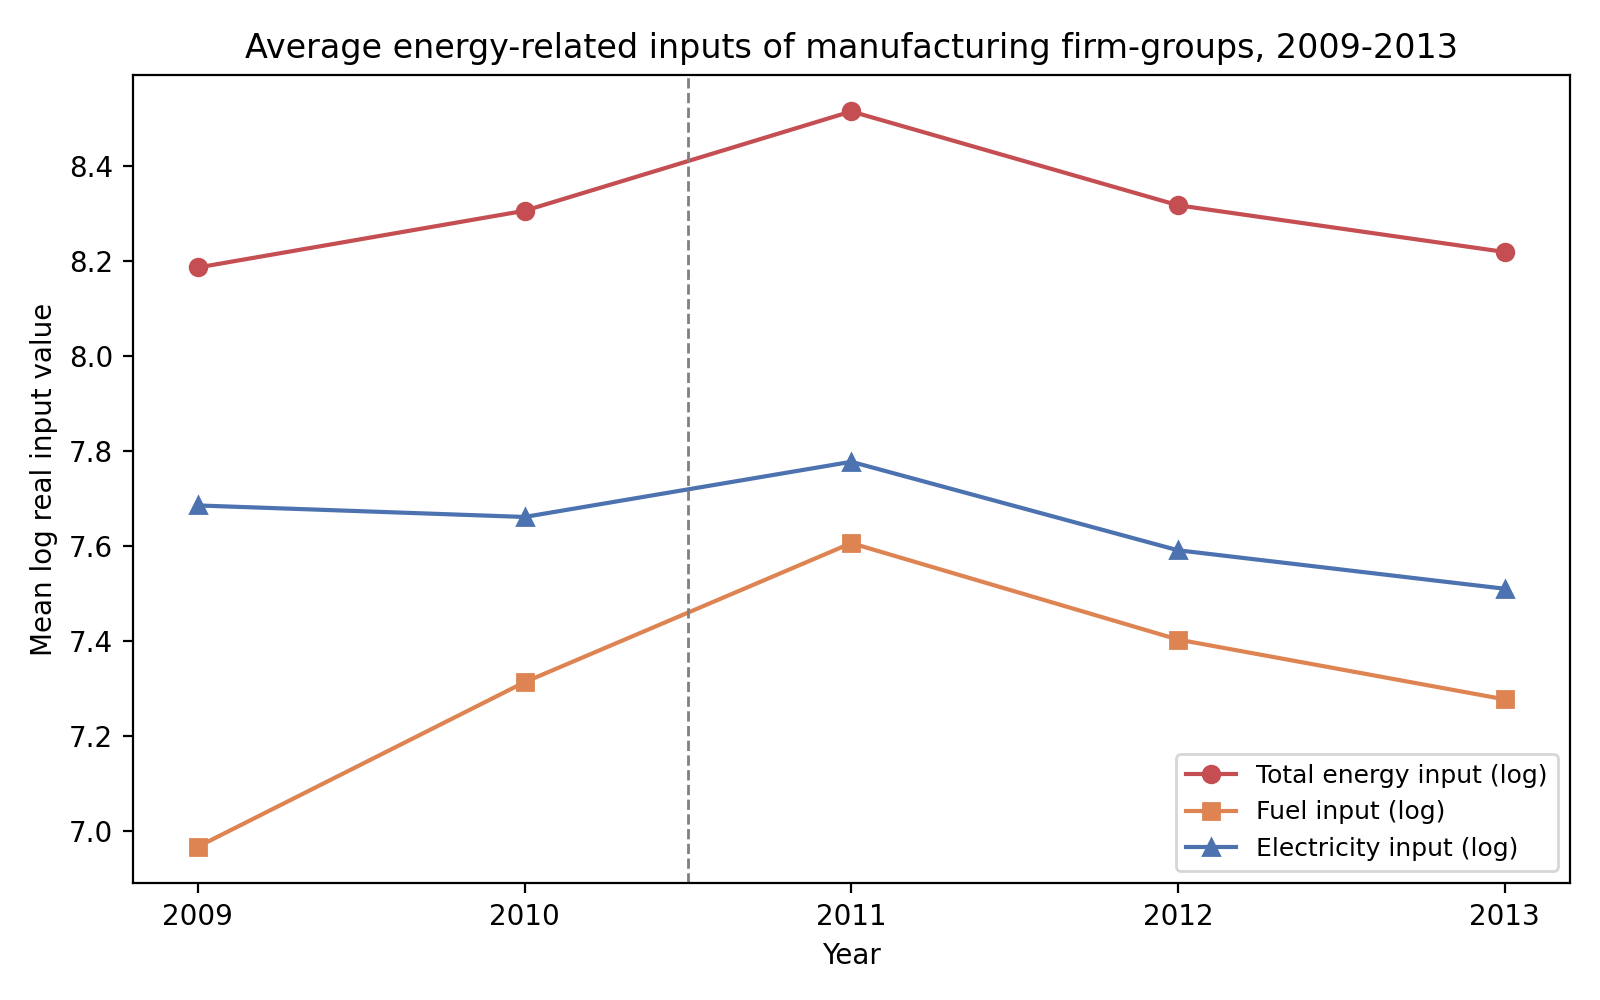
\includegraphics[width=0.75\textwidth]{energy_input_trend.png}%
}{%
    \fbox{\parbox[c][5cm][c]{0.75\textwidth}{\centering محل قرارگیری نمودار روند نهاده‌های انرژی}}%
}
\caption{میانگین لگاریتم هزینه سوخت، برق و کل انرژی در تمامی گروه‌های صنعت--استان، ۲۰۰۹--۲۰۱۳.}
\label{fig:energy}
\end{figure}

\section{راهبرد تجربی}

مدل بازتولید، اثرات ثابت واحد را جذب می‌کند و خطاهای استاندارد را در سطح واحد خوشه‌بندی می‌سازد. صورت تفاضل در تفاضل آن عبارت است از
\begin{equation}
y_{it}=\alpha_i+\beta(\text{Post}_t\times\text{Treat}_i)
+X_{it}'\gamma+\delta\,\text{Sanctions}_t+\rho t+\varepsilon_{it},
\label{eq:binary}
\end{equation}
که در آن $\text{Post}_t$ از سال ۲۰۱۱ به بعد برابر یک است. گروه تیمار شامل صنایع حساس به انرژی است؛ گروه مقایسه نیز صنایع کم‌مصرفی را کنار می‌گذارد که با وجود مصرف مستقیم پایین انرژی، از طریق فلزات و سایر واسطه‌های دارای انرژی نهفته به‌شدت در معرض شوک قرار دارند. چون سیاست بر این گروه مقایسه نیز اثر گذاشته است، $\beta$ یک اثر نسبی است و لزوماً اثر تیمار در مقایسه با نبود اصلاح را نشان نمی‌دهد. علامت و اندازه این تفاوت به اثر واقعی اصلاح در هر دو گروه وابسته است؛ بنابراین برچسب «محافظه‌کارانه» بدون فرض اضافی موجه نیست.

بسط دوز پیوسته مدل زیر را برآورد می‌کند:
\begin{equation}
y_{it}=\alpha_i+\beta_D(\text{Post}_t\times D_i)
+\mu_{s(i),t}+\nu_{p(i),t}+\varepsilon_{it},
\label{eq:dose}
\end{equation}
که در آن $\mu_{s(i),t}$ و $\nu_{p(i),t}$ به‌ترتیب اثرات صنعت دورقمی--سال و استان--سال هستند. ضریب ترجیحی، تغییر پس از اصلاح واحدهایی را مقایسه می‌کند که مواجهه مستقیم پیش از اصلاح آن‌ها یک انحراف معیار تفاوت داشته است؛ شوک‌های سالانه مختص صنعت و استان هم جذب می‌شوند. در یک مشخصات رقابتی، $\beta_I(\text{Post}_t\times I_i)$ برای مواجهه غیرمستقیم اضافه می‌شود، و در مطالعه رویداد (\lr{event study}) برهم‌کنش منفرد دوره پس از اصلاح را با برهم‌کنش‌های دوز--سال جایگزین می‌کنیم و سال ۲۰۱۰ را کنار می‌گذاریم.

برآوردگر از حداقل مربعات معمولیِ تبدیل‌شده درون‌گروهی و تصحیح نمونه کوچک مشابه \lr{\texttt{areg}} استفاده می‌کند. برای استنباط، نوت‌بوک برای مشخصات دوز پیوسته سه سطح خوشه‌بندی (واحد، صنعت، و دوطرفه) را کنار بوت‌استرپ خوشه‌ای وحشی (\lr{wild cluster bootstrap}) مقید به فرض صفر با ۹۹۹ تکرار مقایسه می‌کند -- چون مواجهه مشترک در سطح صنعت می‌تواند خوشه‌بندی واحد را بیش از حد خوش‌بینانه کند. مطالعه رویداد هم تنها مقایسه پیش از تیمارِ موجود در داده را گزارش می‌کند، آن‌طور که دغدغه‌های شناسایی مطرح‌شده در \cite{nakamura2018} توصیه می‌کنند؛ منتها پنل بیش از همین یک مقایسه فراهم نمی‌آورد.

طبقه‌بندی فناوری صنعتی و شدت سرمایه‌گذاری به‌عنوان ابعاد ناهمگنی وارد تحلیل می‌شوند. برای فناوری پایین/متوسط رو به پایین، فناوری متوسط رو به بالا/بالا و مشاهدات بالاتر از آستانه شدت سرمایه‌گذاری، مدل‌های جداگانه برآورد می‌کنیم. این‌ها مقایسه‌های تصادفی‌شده نیستند. آن‌ها نشان می‌دهند ضریب شرطی اصلاح چگونه همراه با ظرفیت تعدیل تغییر می‌کند. استفاده از تشکیل سرمایه به‌عنوان پیامدی جداگانه، امکان تمایز میان یک حاشیه حفاظتی موجود و سرمایه‌گذاری جدید پس از اصلاح را فراهم می‌کند.

\section{نتایج}

\subsection{بازتولید و معنای پارامتر مورد برآورد}

مرحله اعتبارسنجی بازتولید برای هر سه پیامد موفق است؛ الگوی اعداد بازتولیدشده با خلاصه مطالعه مرجع از کاهش حدود ۳، ۷ و ۹ درصدی در تولید، ارزش افزوده و سود سازگار است. برآوردهای قبل--بعد برای کل دوره برابر با ۰٫۰۶۵- برای تولید، ۰٫۱۲۵- برای ارزش افزوده و ۰٫۱۴۸- برای مازاد عملیاتی هستند، با خطاهای استاندارد به‌ترتیب ۰٫۰۱۹، ۰٫۰۳۰ و ۰٫۰۵۵. وقتی دوره پس از اصلاح را فقط به سال ۲۰۱۱ محدود می‌کنیم، ضرایب بزرگ‌تر می‌شوند (۰٫۰۸۲-، ۰٫۱۴۴- و ۰٫۲۰۶-)؛ یعنی انقباض فوری از میانگین واکنش تا سال ۲۰۱۳ شدیدتر است -- الگویی که با انتقال تدریجی قیمت و تعدیل سازگار است.

مدل تفاضل در تفاضل دودویی ترجیحی یک اثر نسبی منفی و بزرگ‌تر در پیامدهای پایین‌دستی برآورد می‌کند: ضریب $\text{Post}\times\text{Treat}$ برابر ۰٫۰۳۴۱- برای تولید، ۰٫۰۷۵۸- برای ارزش افزوده و ۰٫۰۹۵۷- برای مازاد عملیاتی است، که پس از تبدیل دقیق ضرایب لگاریتمی به درصد به کاهش‌های ۳٫۳۵، ۷٫۳۰ و ۹٫۱۲ درصدی می‌رسد ($p=0.043$، $0.0098$، $0.0602$ به‌ترتیب). الگوی جالب توجه این است که بنگاه‌ها به نظر می‌رسد بخشی از فروش خود را حفظ می‌کنند، چون انقباض در ارزش افزوده و مازاد عملیاتی بزرگ‌تر از انقباض در تولید است.

نکته مهمی که باید در نظر گرفت این است که این ضرایب بر نهاده‌های هم‌زمانی شرطی شده‌اند که خودشان هم می‌توانند به اصلاح واکنش نشان دهند. نردبان مشخصات نوت‌بوک دقیقاً همین را آشکار می‌کند: اگر روند خطی را با شاخص‌های سال جایگزین کنیم (و همه نهاده‌ها را نگه داریم)، ضرایب کوچک، مثبت و بی‌معنا می‌شوند؛ و اگر همه کنترل‌های نهاده‌ای را حذف کنیم، برآوردها مثبت و بزرگ‌تر می‌شوند. پس نتیجه بازتولید را باید یک اثر نسبی کنترل‌شده خواند، نه برآوردی مستقل از مدل برای کل هزینه اقتصاد کلان -- چون کنترل‌های پس از تیمار می‌توانند بخشی از خود سازوکار را جذب کنند.

\begin{table}[htbp]
\centering
\caption{برآوردهای اصلی بازتولید و دوز پیوسته}
\label{tab:main}
\begin{tabular}{llrrr}
\toprule
طرح & پیامد & ضریب & خطای استاندارد & مقدار $p$ \\
\midrule
بازتولید دودویی\textsuperscript{\dag} & تولید & $-0.0341$ & 0.0168 & 0.0430 \\
 & ارزش افزوده & $-0.0758$ & 0.0293 & 0.0098 \\
 & مازاد عملیاتی & $-0.0957$ & 0.0509 & 0.0602 \\
\addlinespace
دوز پیوسته ترجیحی\textsuperscript{\ddag} & تولید & $0.0510$ & 0.0209 & 0.0150 \\
 & ارزش افزوده & $0.0121$ & 0.0215 & 0.5750 \\
 & مازاد عملیاتی & $0.0495$ & 0.0377 & 0.1900 \\
\bottomrule
\end{tabular}
\begin{flushright}\footnotesize
توضیحات: ضریب دودویی مربوط به $\text{Post}\times\text{Treat}$ است. ضریب پیوسته مربوط به $\text{Post}\times D_i$ است که در آن $D_i$ مواجهه مستقیم استانداردشده پیش از اصلاح است. خطاهای استاندارد این جدول در سطح واحد خوشه‌بندی شده‌اند؛ بنابراین $p$-مقدارهای بازتولید دودویی دقیقاً برای مشخصات خوشه‌بندی واحد هستند و نباید به‌تنهایی به‌عنوان استنباط مقاوم در برابر هر ساختار همبستگی مکانی یا صنعتی خوانده شوند. اندازه نمونه مدل‌های پیوسته برای سه پیامد به‌ترتیب ۵٬۴۲۶، ۵٬۴۱۳ و ۵٬۲۳۲ است.\\
\dag بازتولید دودویی: Binary reproduction (binary DID).\\
\ddag دوز پیوسته ترجیحی: Preferred continuous dose (continuous treatment intensity).
\end{flushright}
\end{table}

\begin{table}[htbp]
\centering
\caption{کنترل بازتولید در برابر یافته‌های خلاصه‌شده مطالعه مرجع}
\label{tab:replication}
\small
\begin{tabularx}{0.92\textwidth}{lZZZ}
\toprule
پیامد & مطالعه مرجع، یافته تقریبی & بازتولید پروژه & تفاوت در واحد لگاریتمی \\
\midrule
تولید & حدود $-3\%$ & $-0.0341$ ($-3.35\%$) & $-0.0041$ \\
ارزش افزوده & حدود $-7\%$ & $-0.0758$ ($-7.30\%$) & $-0.0058$ \\
مازاد عملیاتی/سود & حدود $-9\%$ & $-0.0957$ ($-9.12\%$) & $-0.0057$ \\
\bottomrule
\end{tabularx}
\begin{flushright}\footnotesize
توضیحات: ستون «مطالعه مرجع» اعداد گرد شده‌ای را نشان می‌دهد که در خلاصه مطالعه زارع‌پور و واگنر (۲۰۲۳) برای کاهش تولید، ارزش افزوده و سود گزارش شده‌اند. ستون «بازتولید پروژه» به ضریب دقیق $\text{Post}\times\text{Treat}$ در جدول اصلی این پروژه اشاره دارد. تفاوت‌ها به دلیل گرد کردن و تفاوت مقیاس گزارش‌اند و نباید به‌عنوان آزمون تفاوت آماری تفسیر شوند.
\end{flushright}
\end{table}

\subsection{مواجهه پیوسته، انتقال و تعدیل}

در مدل پیوسته ترجیحی، افزایش یک انحراف معیار در مواجهه مستقیم با ۰٫۰۵۱ واحد لگاریتمی تولید بیشتر در دوره پس از اصلاح همراه است. ارزش افزوده و مازاد عملیاتی هم مثبت‌اند، منتها دقت آماری کمتری دارند. در نگاه اول این با برآورد منفی مدل دودویی در تناقض به نظر می‌رسد، اما نیست -- چون این دو مدل اصلاً دو چیز متفاوت می‌سنجند. مدل دودویی دو مجموعه ساخته‌شده (حساس به انرژی در برابر کمتر حساس) را مقایسه می‌کند؛ مدل دوز، مسیر پس از اصلاح واحدهایی با سهم‌های متفاوت پیش از اصلاح را پس از حذف شوک‌های صنعت--سال و استان--سال مقایسه می‌کند. نمونه‌ها فرق دارند، سنجه‌های تیمار و کنترل فرق دارند، پس طبیعی است که ضرایب هم چیزهای متفاوتی برآورد کنند.

این شیب مثبت نباید به‌عنوان اثر سودمند افزایش مواجهه تفسیر شود. می‌تواند با سازگاری واحدها، انتقال قیمت به مصرف‌کننده، تغییر ترکیب محصول، موقعیت بالادستی، یا حتی یک عامل مخدوش‌کننده باقیمانده که مدل نگرفته است سازگار باشد. بنابراین تفسیر علّی آن باز است. آنچه با اطمینان بیشتری می‌توان گفت این است که نقطه برآورد مثبت است، اما معناداری آماری آن به‌شدت به شیوه استنباط وابسته است: مقدار $p$ با خوشه‌بندی واحد ۰٫۰۱۵ است، با خوشه‌بندی صنعت به ۰٫۱۹۴ می‌رسد، با خوشه‌بندی دوطرفه صنعت--استان ۰٫۲۲۲ می‌شود، و در بوت‌استرپ وحشی صنعت دوباره به ۰٫۰۰۹ برمی‌گردد. برآورد نقطه‌ای در همه این حالت‌ها ثابت می‌ماند؛ آنچه تغییر می‌کند عدم قطعیت اطراف آن است -- و این خودش به تعداد کم خوشه‌های صنعتی برمی‌گردد.

\begin{figure}[htbp]
\centering
\IfFileExists{fig4_inference.png}{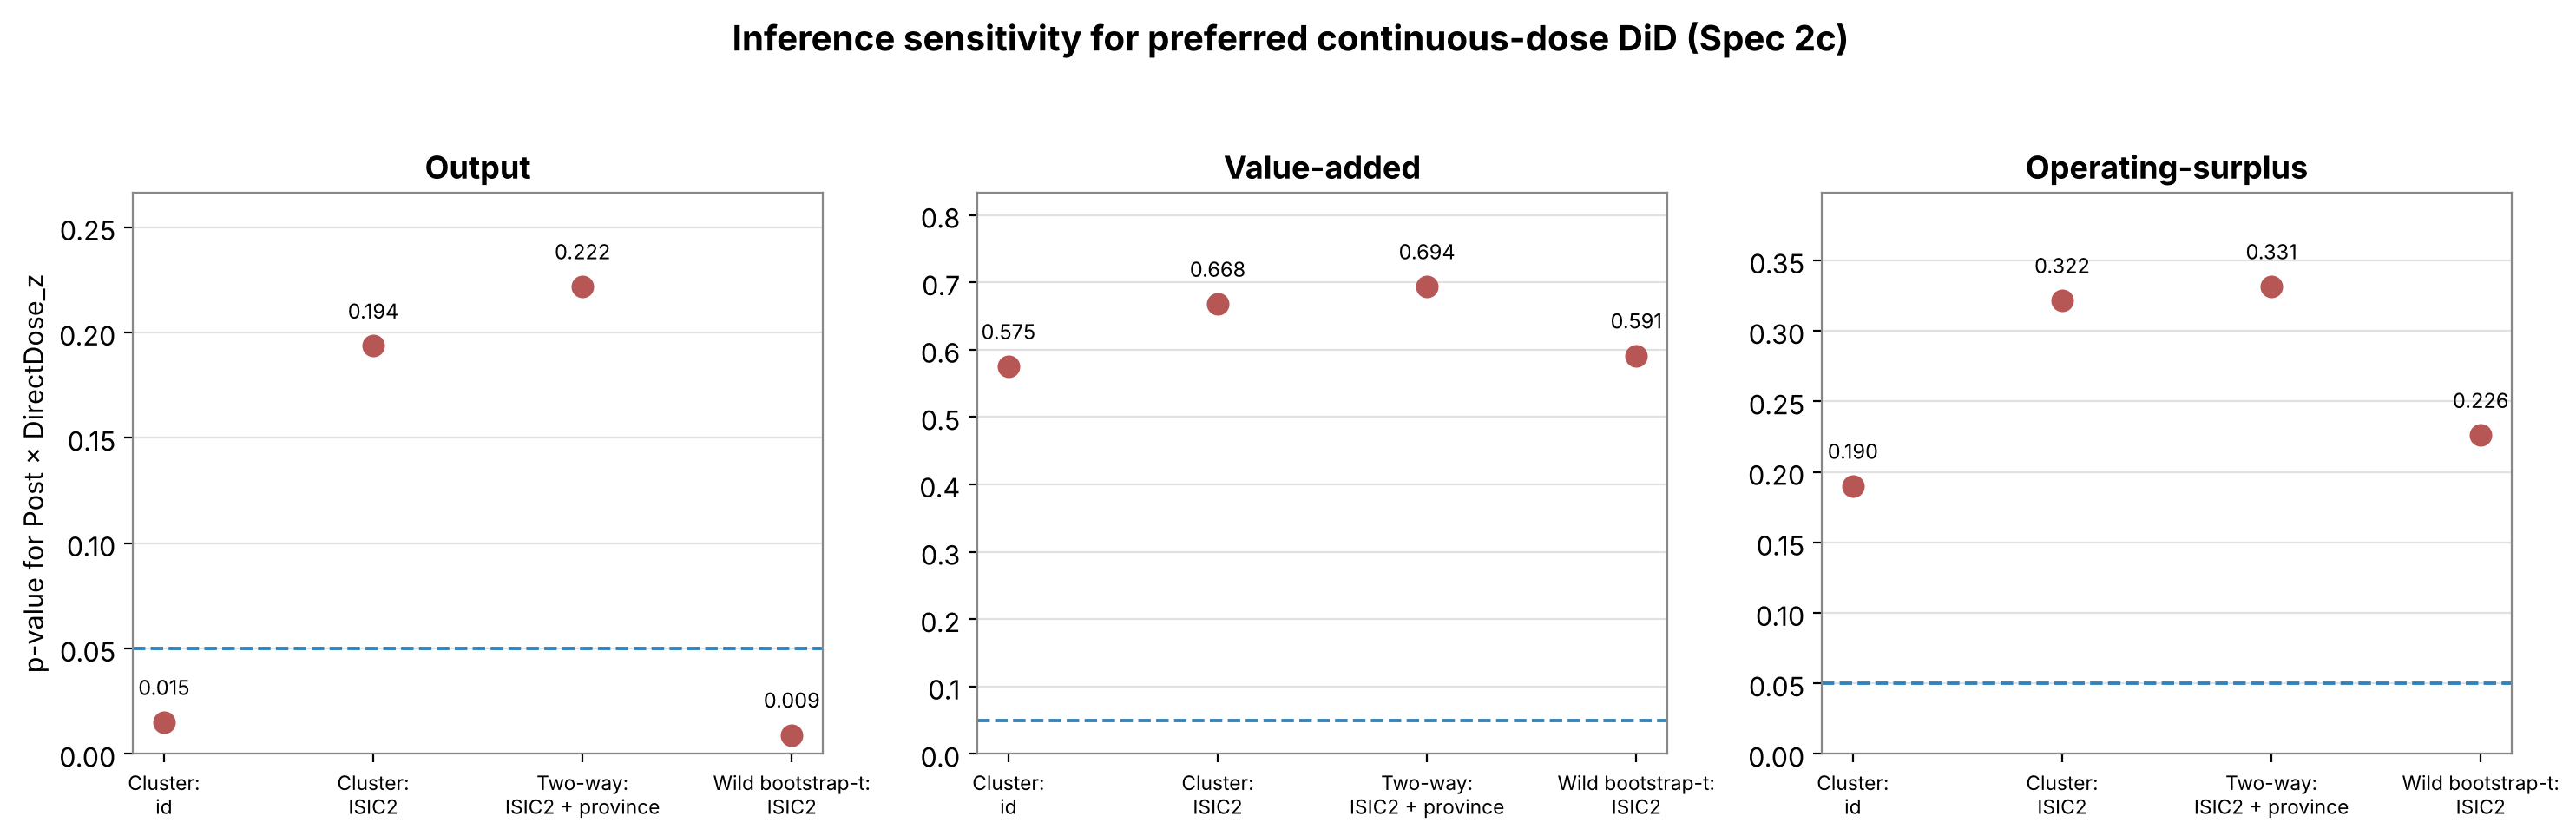
\includegraphics[width=\textwidth]{fig4_inference.png}}{\fbox{\parbox[c][5cm][c]{0.92\textwidth}{\centering محل قرارگیری نمودار حساسیت استنباطی نوت‌بوک}}}
\caption{حساسیت استنباطی در مشخصات ترجیحی دوز پیوسته}
\label{fig:inference}
\begin{flushright}\footnotesize
توضیحات: شکل مقادیر $p$ ضریب $\text{Post}\times\text{DirectDose}$ را تحت خوشه‌بندی واحد، خوشه‌بندی صنعت، خوشه‌بندی دوطرفه صنعت و استان و روش بوت‌استرپ وحشی صنعت گزارش می‌کند. خط‌چین سطح ۵ درصد را نشان می‌دهد.
\end{flushright}
\end{figure}

بررسی پویایی دوز--زمان و پیش‌روند، با توجه به تنها یک دوره پیش از اصلاح، اطمینان محدودی می‌دهد. نسبت به سال ۲۰۱۰، ضرایب دوز در سال ۲۰۰۹ برابر ۰٫۰۲۴ برای تولید، ۰٫۰۴۵ برای ارزش افزوده و ۰٫۰۲۰ برای مازاد عملیاتی است، با مقادیر $p$ به‌ترتیب ۰٫۳۸۲، ۰٫۱۲۴ و ۰٫۶۴۴. عدم رد فرض صفر در اینجا فقط بر پایه یک مقایسه پیش از دوره است، پس این شواهد آزمون قدرتمندی برای روند موازی (\lr{parallel trends}) نیست -- درست است که پیش‌روند متفاوت و بزرگی دیده نمی‌شود، ولی این آزمون نمی‌تواند نبودش را اثبات کند.

\begin{figure}[htbp]
\centering
\IfFileExists{fig1_event_study.png}{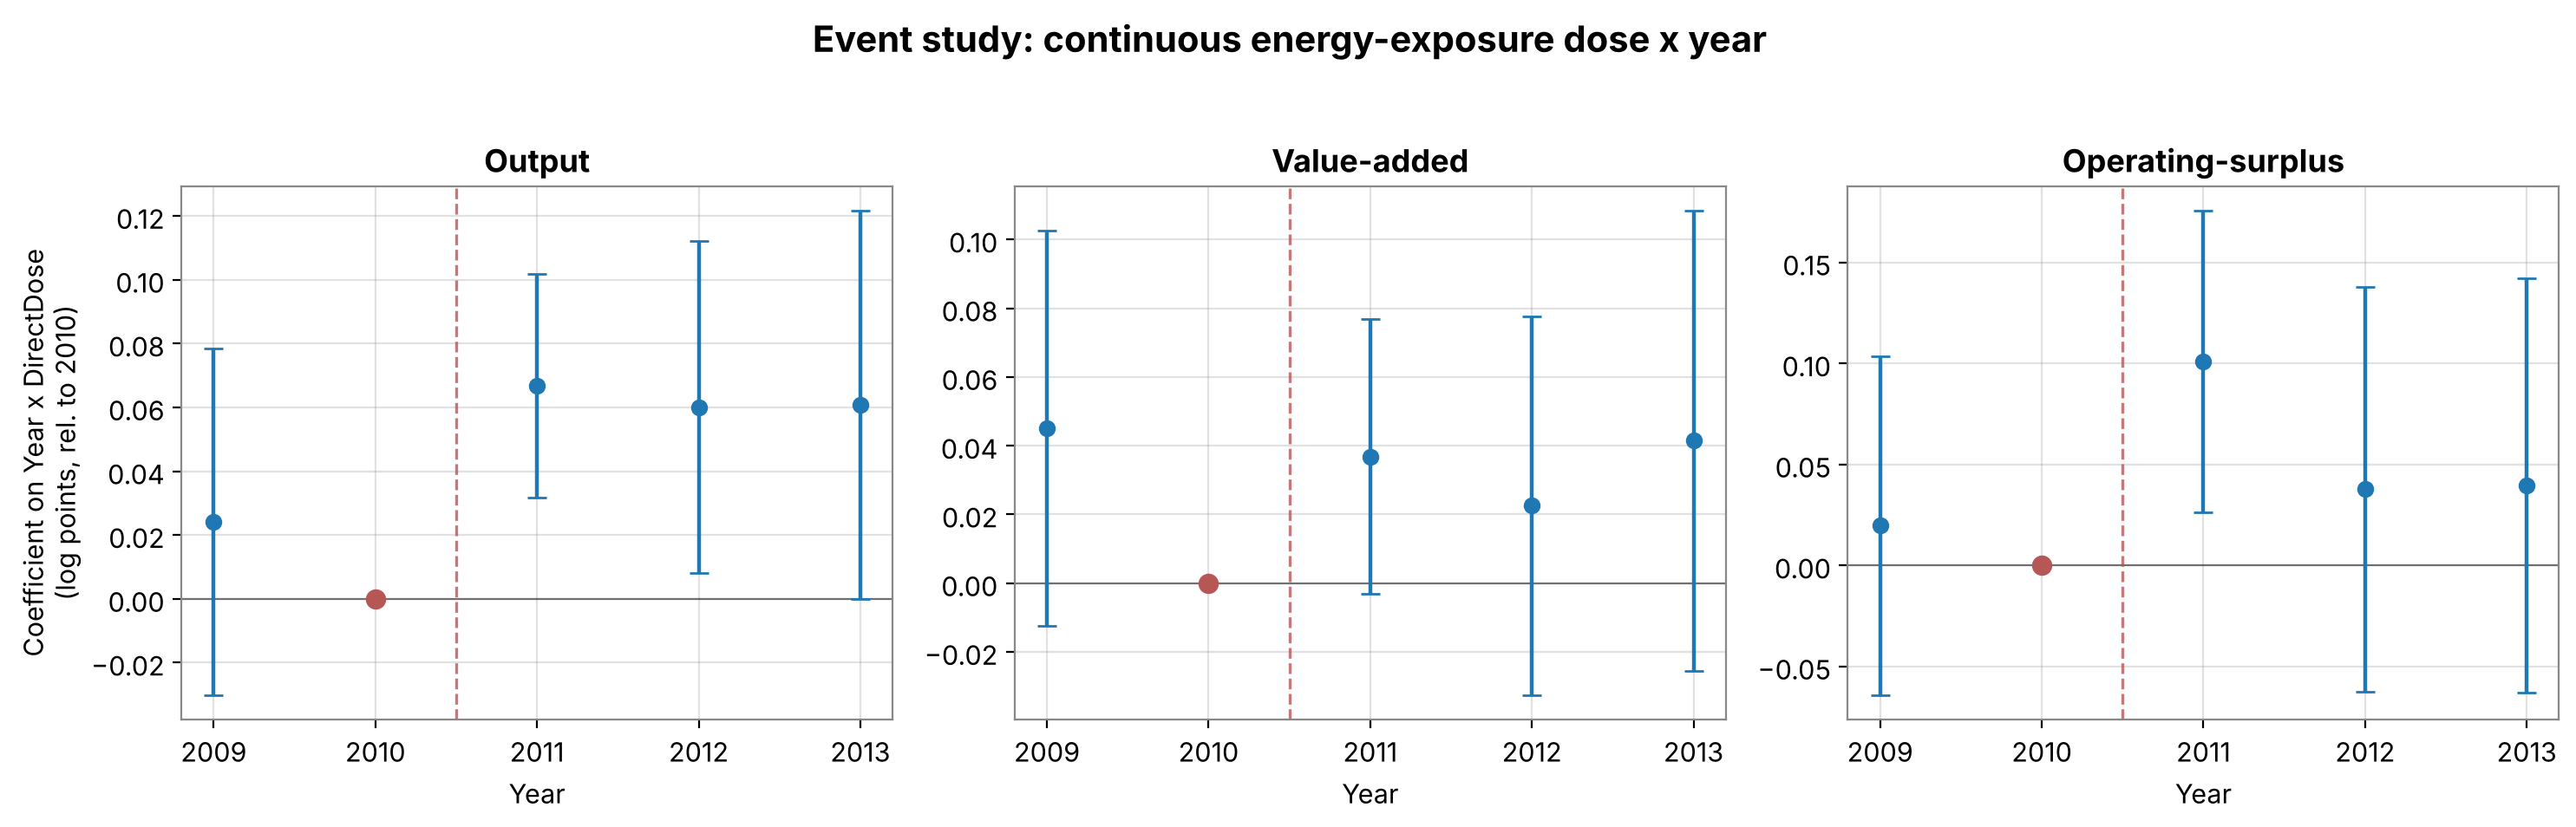
\includegraphics[width=\textwidth]{fig1_event_study.png}}{\fbox{\parbox[c][5cm][c]{0.92\textwidth}{\centering محل قرارگیری نمودار مطالعه رویداد نوت‌بوک}}}
\caption{برآوردهای مطالعه رویداد برای مواجهه پیوسته با انرژی پیش از اصلاح}
\label{fig:event-study}
\begin{flushright}\footnotesize
توضیحات: نمودارها ضرایب دوز--سال و فاصله‌های اطمینان ۹۵ درصد را برای تولید، ارزش افزوده و مازاد عملیاتی نشان می‌دهند. سال حذف‌شده ۲۰۱۰ است؛ خط‌چین عمودی دوره‌های پیش و پس از اصلاح را جدا می‌کند.
\end{flushright}
\end{figure}

وقتی دوزهای مستقیم و غیرمستقیم را با هم وارد مدل می‌کنیم، فقط مواجهه مستقیم تولید را پیش‌بینی می‌کند ($0.0606$، $p=0.024$)؛ جانشین غیرمستقیم چنین رابطه‌ای ندارد ($0.0204$، $p=0.543$). برای ارزش افزوده و مازاد عملیاتی ماجرا برعکس است -- هر دو ضریب مثبت‌اند، ولی این‌بار ضریب غیرمستقیم بزرگ‌تر است، و آزمون برابری شیب‌ها برای ارزش افزوده رد می‌شود ($p=0.0006$) و برای مازاد عملیاتی روی مرز معناداری می‌ایستد ($p=0.0588$). چون همبستگی دو دوز تبدیل‌شده ۰٫۵۲۲- است، هم‌زمانی این دو سنجه می‌تواند دقت برآورد ضرایب مشترک را کاهش دهد و تفسیر جداگانه آن‌ها را دشوارتر کند. باید هم در نظر داشت که سنجه غیرمستقیم فقط وابستگی مخارج را می‌بیند، نه شدت واقعی انرژی بالادستی را -- بنابراین کشش ساختاری انتقال قیمت را نمی‌تواند شناسایی کند.

رگرسیون‌های حاشیه تعدیل یک الگوی نسبتاً دقیق نشان می‌دهند: تنها مخارج مواد اولیه است که به‌طور معناداری واکنش نشان می‌دهد -- به‌ازای یک انحراف معیار مواجهه مستقیم، ۰٫۱۰۸ واحد لگاریتمی افزایش می‌یابد ($p=0.0085$). بقیه (مخارج انرژی، تشکیل سرمایه، جبران خدمات کارکنان، تعداد بنگاه‌ها، خدمات تولیدی) از صفر قابل تفکیک نیستند؛ ضریب تشکیل سرمایه مشخصاً ۰٫۰۱۸۲- با $p=0.695$ است. این الگو با ترکیب مجدد نهاده‌ها در کوتاه‌مدت سازگارتر از یک واکنش سریع موجودی سرمایه است، اما به‌تنهایی یک سازوکار علّی را اثبات نمی‌کند. نتیجه به دوز مبتنی بر رتبه هم حساس نیست -- همان جهت را نشان می‌دهد -- و وقتی نمونه را فقط به واحدهای مشاهده‌شده در هر دو سال پیش از اصلاح محدود می‌کنیم، ضریب تولید همچنان مثبت می‌ماند ($0.0451$، $p=0.0304$).

\begin{figure}[htbp]
\centering
\begin{minipage}{0.48\textwidth}
\centering
\IfFileExists{fig2_dose_response.png}{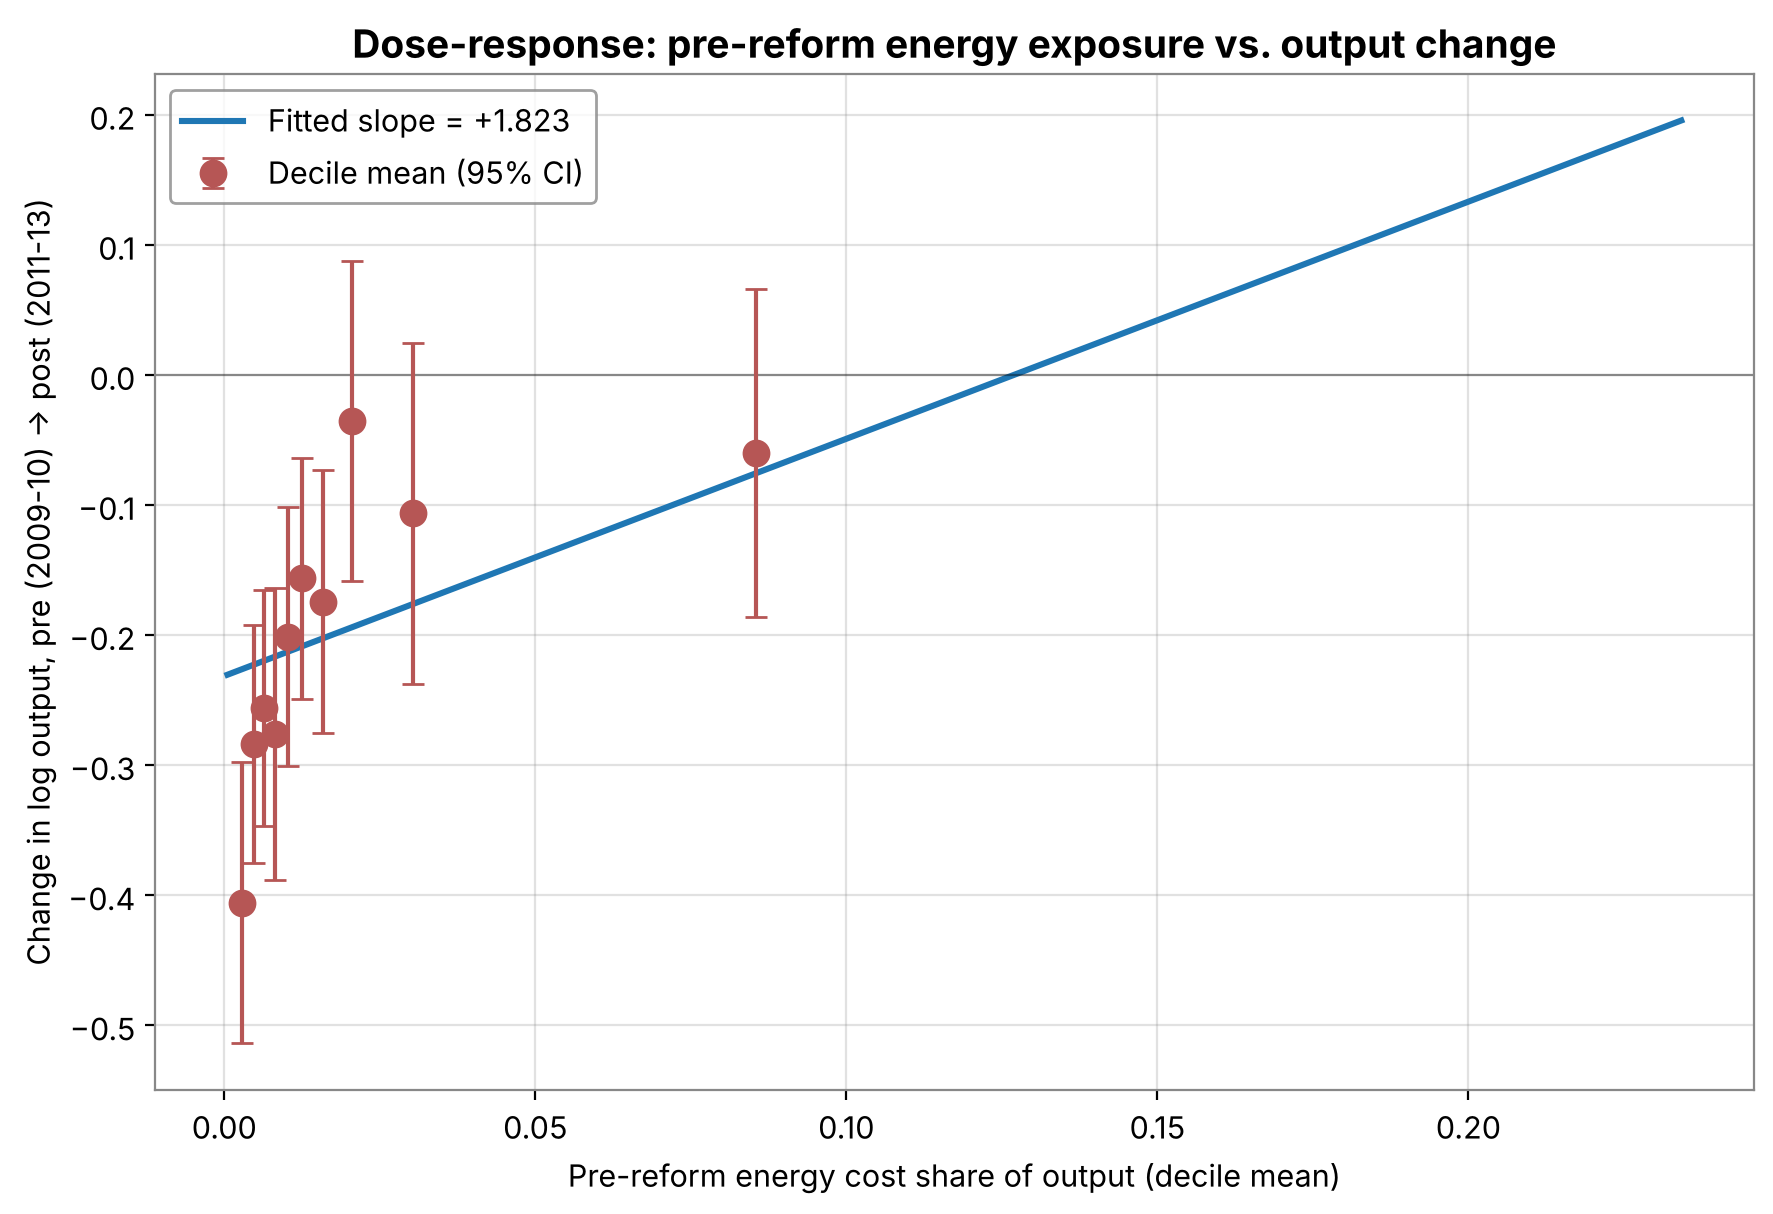
\includegraphics[width=\linewidth]{fig2_dose_response.png}}{\fbox{\parbox[c][4cm][c]{0.9\linewidth}{\centering محل قرارگیری نمودار دوز--پاسخ نوت‌بوک}}}
\end{minipage}\hfill
\begin{minipage}{0.48\textwidth}
\centering
\IfFileExists{fig3_adjustment_margins.png}{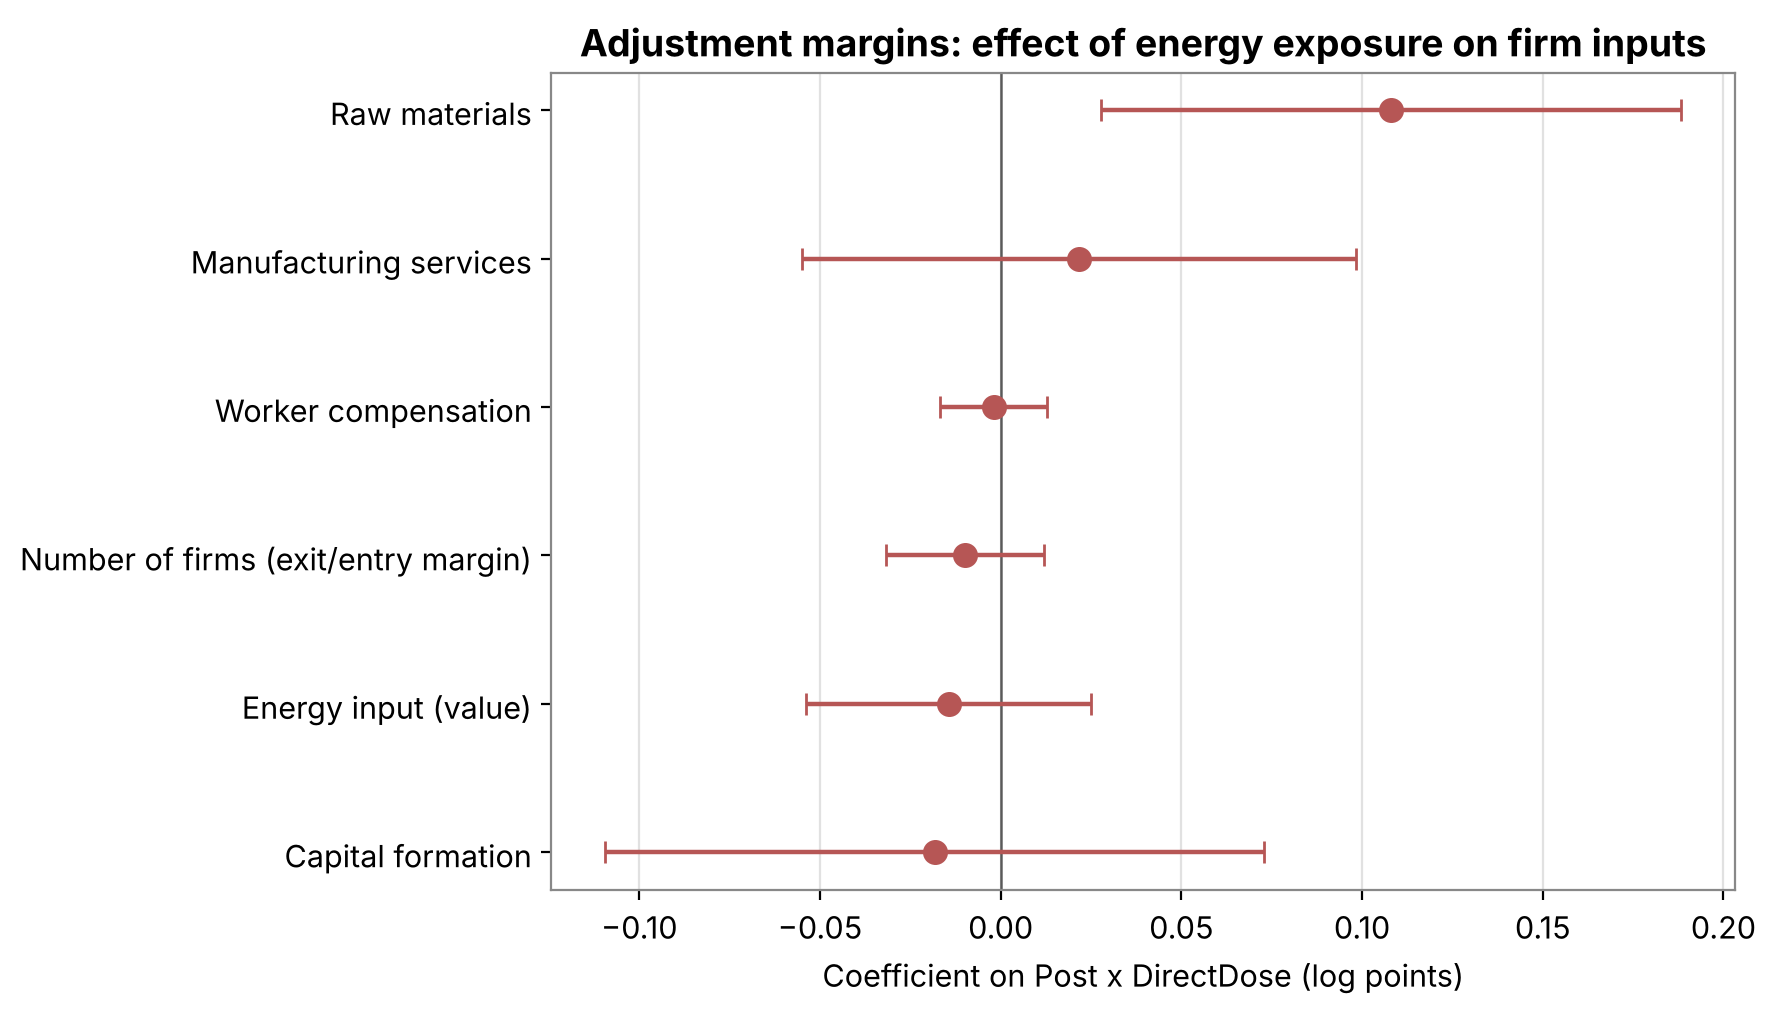
\includegraphics[width=\linewidth]{fig3_adjustment_margins.png}}{\fbox{\parbox[c][4cm][c]{0.9\linewidth}{\centering محل قرارگیری نمودار حاشیه‌های تعدیل نوت‌بوک}}}
\end{minipage}
\caption{رابطه دوز--پاسخ و حاشیه‌های تعدیل}
\label{fig:mechanisms}
\begin{flushright}\footnotesize
توضیحات: نمودار سمت چپ سهم مستقیم هزینه انرژی پیش از اصلاح را به تغییر در لگاریتم تولید مرتبط می‌کند و میانگین دهک‌ها را با فاصله‌های اطمینان ۹۵ درصد نشان می‌دهد. نمودار سمت راست ضرایب و فاصله‌های اطمینان ۹۵ درصد $\text{Post}\times\text{DirectDose}$ را برای شش پیامد تعدیل گزارش می‌کند.
\end{flushright}
\end{figure}

\subsection{فناوری صنعتی و شدت سرمایه‌گذاری}

تفکیک بر اساس طبقه‌بندی فناوری صنعتی از نظر اقتصادی چشمگیر است. در گروه‌های فناوری پایین و متوسط رو به پایین، ضرایب اصلاح در طرح مرجع ۰٫۰۷۸- برای تولید، ۰٫۱۴۲- برای ارزش افزوده و ۰٫۱۶۱- برای مازاد عملیاتی است -- یعنی زیان‌هایی حدود ۷٫۵، ۱۳٫۲ و ۱۴٫۹ درصد. در گروه‌های فناوری متوسط رو به بالا و بالا این ضرایب به ۰٫۰۲۶-، ۰٫۰۷۸- و ۰٫۱۳۴- می‌رسند و در سطوح متعارف معنادار نیستند. الگو با این احتمال سازگار است که صنایعی که در طبقات فناوری بالاتر قرار می‌گیرند مجموعه جانشینی گسترده‌تری داشته باشند، بهتر پایش می‌کنند یا تجهیزات کاراتری در اختیار دارند. با این حال نمی‌شود از این یافته نتیجه گرفت که فناوری به‌تنهایی سبب تاب‌آوری است، چون فناوری در سطح صنعت تخصیص یافته و با موقعیت بنگاه در شبکه تولید همبسته است -- ممکن است چیز دیگری پشت این رابطه باشد.

شدت سرمایه‌گذاری تصویر مکملی به دست می‌دهد. گروه‌هایی که نسبت تشکیل سرمایه ثابت به تولیدشان از ۰٫۰۶ بیشتر است، در مدل زیرگروهی قبل--بعد زیان برآوردی ۴٫۳ درصد در تولید، ۹٫۸ درصد در ارزش افزوده و ۱۰٫۶ درصد در مازاد عملیاتی نشان می‌دهند -- کوچک‌تر از زیان‌های متناظر برای کل نمونه در \citet{zarepour2023}، هرچند این برآوردهای زیرگروهی خودشان دقت چندانی ندارند. تفسیر قابل‌قبول این است که این الگو با این تفسیر سازگار است که واحدهای با شدت سرمایه‌گذاری بالاتر ممکن است ظرفیت تعدیل متفاوتی داشته باشند؛ برای مثال، دسترسی به منابع مالی یا تجهیزات کارآمدتر می‌تواند نقش داشته باشد. اما تشکیل سرمایه خودش نسبت به دوز واکنش معناداری نشان نمی‌دهد. این یافته صرفاً با این تفسیر سازگار است که بخشی از تفاوت واکنش از ظرفیت موجود ناشی شود؛ نشان نمی‌دهد که این سازوکار حتماً از سرمایه‌گذاری گذشته می‌آید و سرمایه‌گذاری جدید را نیز رد نمی‌کند. چون نسبت شدت سرمایه‌گذاری در طول زمان تغییر می‌کند، علیت معکوس (\lr{reverse causality}) و انتخاب نمونه هم‌چنان محتمل باقی می‌مانند.

\begin{table}[htbp]
\centering
\caption{ناهمگنی فناوری صنعتی و شدت سرمایه‌گذاری}
\label{tab:heterogeneity}
\small
\begin{tabularx}{\textwidth}{lZZZ}
\toprule
پیامد & فناوری پایین/متوسط رو به پایین & فناوری متوسط رو به بالا/بالا & شدت سرمایه‌گذاری بالا \\
\midrule
تولید & $-0.078^{***}$ & $-0.026$ & $-0.044$ \\
 & $(0.023)$ & $(0.027)$ & $(0.055)$ \\
ارزش افزوده & $-0.142^{***}$ & $-0.078$ & $-0.103$ \\
 & $(0.036)$ & $(0.057)$ & $(0.099)$ \\
مازاد عملیاتی & $-0.161^{**}$ & $-0.134$ & $-0.112$ \\
 & $(0.066)$ & $(0.103)$ & $(0.217)$ \\
\bottomrule
\end{tabularx}
\begin{flushright}\footnotesize
توضیحات: خطاهای استاندارد داخل پرانتز آمده‌اند. نمونه‌های فناوری برای سه پیامد در گروه فناوری پایین به‌ترتیب شامل ۳٬۵۴۱/۳٬۵۲۹/۳٬۴۱۵ مشاهده و در گروه فناوری بالا شامل ۱٬۳۲۰/۱٬۳۱۹/۱٬۲۷۸ مشاهده‌اند. نمونه‌های شدت سرمایه‌گذاری بالا شامل ۱٬۱۳۳/۱٬۱۲۶/۱٬۰۸۱ مشاهده‌اند. $^{**}p<0.05$، $^{***}p<0.01$.
\end{flushright}
\end{table}

\section{مقایسه با مقاله پایه}

دو مطالعه از نظر رویداد سیاستی، پنل، پیامدها، منطق اثرات ثابت، طبقه‌بندی تیمار--کنترل و سه مسیر انتقال مشترک‌اند. تفاوت‌های اصلی آن‌ها به اندازه‌گیری، قابلیت بازتولید و نحوه سازمان‌دهی ناهمگنی مربوط می‌شود.

\begin{table}[htbp]
\centering
\caption{مقایسه با مطالعه اصلی الهام‌بخش}
\label{tab:comparison}
\begin{tabularx}{\textwidth}{>{\raggedleft\arraybackslash\bfseries}p{0.22\textwidth}YY}
\toprule
بُعد مقایسه & زارع‌پور و واگنر (۲۰۲۳) & پروژه حاضر \\
\midrule
مواجهه اصلی & گروه‌های دودویی حساس و کمتر حساس به انرژی & سهم‌های پیوسته مخارج مستقیم و غیرمستقیم پیش از اصلاح، در کنار بازتولید دودویی \\
کنترل‌های زمانی & روند خطی و جانشین تحریم در مدل اصلی & بازتولید مدل اصلی، به‌علاوه اثرات صنعت--سال و استان--سال در مدل دوز ترجیحی \\
اعتبارسنجی & برآوردهای منتشرشده و جدول‌های حساسیت & مرحله صریح بازتولید عددی پیش از پذیرش بسط‌ها \\
استنباط & خطاهای استاندارد خوشه‌بندی‌شده در سطح واحد & مقایسه خوشه‌بندی واحد، صنعت، دوطرفه و بوت‌استرپ وحشی \\
سازوکارها & استنباط مسیرهای مستقیم، غیرمستقیم و تقاضا از الگوهای زیرگروهی & رقابت دوز مستقیم و غیرمستقیم و رگرسیون شش حاشیه تعدیل \\
فناوری صنعتی و شدت سرمایه‌گذاری & برآوردهای زیرگروهی فناوری و شدت سرمایه‌گذاری بالا از پیش وجود دارند & این ابعاد در تفسیر یکپارچه جایگاهی مرکزی دارند و به شواهد دوز--پاسخ و تعدیل پیوند می‌خورند \\
\bottomrule
\end{tabularx}
\end{table}

زارع‌پور و واگنر هم تفکیک‌های فناوری و شدت سرمایه‌گذاری بالا را گزارش می‌کنند، اما درون بخش گسترده‌تری درباره ناهمگنی. تفاوت اصلی ما با آن‌ها در جایگاهی است که به این دو متغیر می‌دهیم: در این پروژه، طبقه‌بندی فناوری صنعتی و شدت سرمایه‌گذاری محور اصلی تفسیر تجربی‌اند، نه یک تفکیک تکمیلی. از آن‌ها برای سه کار استفاده می‌کنیم -- ارزیابی پشتیبانی مشترک، تفسیر ضرایب دوز پیوسته، و تمایز میان ظرفیت تعدیل موجود و سرمایه‌گذاری پس از اصلاح. البته ادعا نداریم این متغیرها در مطالعه زارع‌پور غایب بودند؛ فقط نقششان آن‌جا تفکیک تکمیلی است و این‌جا متغیر توضیحی مرکزی.

این تأکید برای شناسایی هم مهم است، نه فقط برای تفسیر. وضعیت تیمار در میان گروه‌های فناوری به‌صورت نامتوازن توزیع شده، در حالی که ظرفیت تعدیل با مواجهه و پیامدهای پس از اصلاح همبستگی دارد -- یک ضریب تجمیعی می‌تواند توابع واکنش کاملاً متفاوتی را پشت خودش پنهان کند. شدت سرمایه‌گذاری هم مواجهه را از ظرفیت تعدیل جدا می‌کند: سهم انرژی برابر لزوماً به معنای فضای مالی، عمر ماشین‌آلات یا موجودی سرمایه برابر نیست. نتایج زیرگروهی همان ناهمگنی‌ای را روشن می‌کنند که اثر متوسط تیمار پشت خودش مخفی نگه می‌دارد.

\section{محدودیت‌ها}

چند محدودیت واقعی وجود دارد که باید صریح گفته شوند. اول، اصلاح سراسری بود -- گروه مقایسه کمتر در معرض شوک قرار داشت، اما تیمارنشده نبود، پس ضریب دودویی ماهیتی نسبی دارد نه مطلق. سرریزها از مسیر قیمت نهاده‌های واسطه‌ای و تقاضای کل هم برداشت لفظی از فرض ثبات تیمار (\lr{SUTVA}) را زیر سؤال می‌برند. طرح دوز پیوسته وابستگی به یک آستانه طبقه‌بندی واحد را کم می‌کند، ولی مواجهه برون‌زا نمی‌سازد؛ سهم‌های انرژی پیش از اصلاح می‌توانند با روندهای مشاهده‌نشده، قدرت بازار، موقعیت بالادستی یا توان انتقال هزینه به قیمت محصول همبسته باشند.

دوم، دسترسی ما فقط به دو سال پیش از اجرای سیاست محدود است. این یعنی مطالعه رویداد فقط یک مقایسه پیش از اصلاح دارد (۲۰۰۹ در برابر ۲۰۱۰) که نمی‌تواند پیش‌روندهای غیرخطی، پیش‌بینی سیاست، یا همگرایی میان‌مدت را نشان بدهد. همین کوتاهی افق زمانی یکی از دلایل اصلی است که مدل‌های پایه و فناوری/شدت سرمایه‌گذاری اثر ثابت سال ندارند: با دو سال پیش از سیاست و سه سال پس از آن، چهار متغیر مجازی سال روی یک پنل پنج‌ساله از نظر زمانی بسیار پرپارامتر است و در چارچوب تصریح این مطالعه عملاً می‌تواند به بیش‌برازش منجر شود؛ همچنین زمان‌بندی سیاست را مکانیکی برازش می‌دهد و می‌تواند بخش بزرگی از تغییر پس از اصلاح را جذب کند. به همین دلیل جانشین تحریم و روند خطی مقاله مبنا را نگه داشتیم -- و نردبان مشخصات نوت‌بوک هم نشان می‌دهد که تعویض روند با شاخص‌های سال ضرایب را محسوس تغییر می‌دهد. این انتخاب شناسایی و قابلیت مقایسه را حفظ می‌کند، اما مدل پایه همچنان در برابر خطای تصریح شوک‌های مشترک آسیب‌پذیر می‌ماند.

سوم، مدل ترجیحی دوز پیوسته به شکل دیگری با اثرات ثابت کنار می‌آید: اثرات ثابت صنعت دورقمی--سال و استان--سال دارد که خودشان از پیش شاخص‌های مشترک سال را پوشش می‌دهند، پس یک اثر سال جداگانه در این‌جا زائد و هم‌خط می‌بود. بازتولید از یک روند کم‌پارامتر استفاده کرده و بسط از ساختار زمانی تودرتو -- ولی داده‌ها نه از روندهای مختص واحد پشتیبانی می‌کنند و نه از یک مطالعه رویداد طولانی پیش از سیاست.

چهارم، و شاید مهم‌تر از همه، همپوشانی تیمار در میان واحدهای کم‌فناوری ضعیف است: گروه فناوری پایین/متوسط رو به پایین فقط ۵۹ واحد کنترل در برابر ۹۰۵ واحد تیمار دارد (۲۱۷ در برابر ۳٬۸۶۱ مشاهده)، یعنی کنترل حدود ۶٫۱ درصد واحدها و ۵٫۳ درصد مشاهدات این زیرنمونه را تشکیل می‌دهد. خطاهای استاندارد خوشه‌بندی‌شده این کمبود پشتیبانی مشترک را حل نمی‌کنند، و برآورد کم‌فناوری می‌تواند تحت تأثیر یک گروه مقایسه کوچک و غیرمعمول باشد. وزن‌دهی مجدد یا تطبیق هم فقط با کنار گذاشتن بخش بزرگی از نمونه تیمار ممکن است، که خودش جمعیت هدف را عوض می‌کند -- به همین خاطر این برآورد زیرنمونه‌ای را باید با احتیاط خواند.

یک نگرانی دیگر این است که چند تا از کنترل‌ها می‌توانند متغیر میانجی باشند. انرژی، مواد اولیه، جبران خدمات و تشکیل سرمایه خودشان به سیاست واکنش نشان می‌دهند؛ گنجاندنشان در معادله~\eqref{eq:binary} پس، تحت مفروضات قوی، یک اثر مستقیم کنترل‌شده را برآورد می‌کند نه اثر کل را -- چیزی که تغییر علامت‌ها در نردبان مشخصات هم نشانش می‌دهد. پژوهش بعدی بهتر است مدل‌های اثر کل را با متغیرهای از پیش مشخص جدا کند و رگرسیون‌های سازوکار را در گزارشی جداگانه بیاورد.

اندازه‌گیری فناوری و شدت سرمایه‌گذاری هم محدودیت خودش را دارد. فناوری صرفاً یک طبقه‌بندی صنعتی \lr{OECD} است، نه سنجه‌ای مستقیم از ماشین‌آلات، ثبت اختراع، کیفیت مدیریت یا بهره‌وری انرژی؛ سنجه شدت سرمایه‌گذاری هم یک نسبت متغیر جریان به تولید است، نه موجودی سرمایه آغاز دوره یا سنجه پاک از نقدینگی -- و این نسبت خودش در طول زمان تغییر می‌کند و می‌تواند به عملکرد واکنش نشان دهد. این متغیرها همبسته‌های اطلاعاتی ظرفیت تعدیل‌اند، نه شناساگر آثار علّی فناوری یا موجودی سرمایه. داده‌های ترازنامه‌ای بنگاه‌محور، عمر ماشین‌آلات، ثبت اختراع و مقادیر فیزیکی انرژی می‌توانستند اندازه‌گیری را بهتر کنند.

در نهایت، خود استنباط آماری قطعی نیست. خوشه‌بندی واحد برای ضریب پیوسته تولید معناداری می‌سازد، اما خوشه‌بندی صنعت و دوطرفه این نتیجه را نمی‌دهند؛ بوت‌استرپ وحشی فرض صفر را رد می‌کند اما روی تعداد کمی خوشه صنعتی تکیه دارد. بنابراین، نتیجه مثبت دوز پیوسته باید یک یافته حساس به استنباط و نه یک اثر علّی قطعی تلقی شود. پنل هم نامتوازن است -- ۱۲۳ واحد دوز پیش از اصلاح ندارند و مازاد عملیاتی نسبت به تولید مشاهدات مفقود بیشتری دارد -- و تحریم‌های ۲۰۱۲ هم درست با دوره پس از اصلاح هم‌زمان شده‌اند. جمع همه این‌ها می‌گوید برآوردها شواهد شبه‌آزمایشی منضبطی‌اند، نه یک تجزیه علّی قطعی.

\section{دلالت‌های سیاستی و جمع‌بندی}

چه چیزی از این کار برای سیاست‌گذاری می‌ماند؟ اول این‌که طراحی اصلاح یارانه را نمی‌شود صرفاً روی متوسط شدت انرژی بنا کرد -- باید هم مصرف مستقیم انرژی بنگاه‌ها و هم وابستگی‌شان به عرضه‌کنندگان انرژی‌بر را در نظر گرفت. تعدیل تدریجی و از پیش اعلام‌شده قیمت به بنگاه‌ها فرصت می‌دهد ماشین‌آلات، قراردادها و قیمت محصولاتشان را عوض کنند؛ و تأمین مالی موقت برای ارتقای بهره‌وری، مخصوصاً برای تولیدکنندگان کم‌فناوری و دارای محدودیت سرمایه، می‌تواند جایگزین هدفمندتری برای حفظ دائمی قیمت‌های پایین انرژی باشد؛ بااین‌حال این پروژه مستقیماً اثربخشی نسبی این دو سیاست را برآورد نمی‌کند. چون واکنش تشکیل سرمایه در سه سال اول پس از اصلاح ضعیف بود، نتایج با این ایده سازگارند که سیاست‌های اعتباری و پذیرش فناوری پیش از اصلاح یا هم‌زمان با آن اجرا شوند؛ این توصیه نیز فراتر از شواهد علّی مستقیم این پروژه است.

نکته روش‌شناختی مهم‌تری هم هست: طرح دودویی زیان‌های نسبی معناداری پیدا می‌کند، اما طرح دوز پیوسته رتبه‌بندی شرطی متفاوتی می‌دهد و حساسیت شدید به شیوه خوشه‌بندی را آشکار می‌کند. این دو یافته، همان‌طور که تکرار شد، به دو پرسش متفاوت جواب می‌دهند -- و یک ارزیابی معتبر باید بگوید دقیقاً چه پارامتری را برآورد کرده، اثر کل را از سازوکار کنترل‌شده جدا کند، و عدم قطعیت را متناسب با ساختار وابستگی داده نشان دهد.

در نهایت، طبقه‌بندی فناوری صنعتی و شدت سرمایه‌گذاری دو متغیر سازمان‌دهنده مهم برای فهم این تعدیل ناهمگن هستند. فناوری صنعتی بالاتر ممکن است با امکان جانشینی بیشتری همراه باشد، و شدت سرمایه‌گذاری بالاتر می‌تواند با ظرفیت تعدیل متفاوتی همراه شود؛ بااین‌حال هر دو سنجه در سطح صنعت--استان هستند و اثر علّی فناوری یا موجودی سرمایه را شناسایی نمی‌کنند. شواهد ما با این تصویر سازگار است -- بدون این‌که آن را اثبات کند. سهم اصلی این پروژه پیوند زدن مواجهه به ظرفیت تعدیل بوده، و هم‌زمان نشان دادن مرز دقیق ادعاهایی که این پنل خاص می‌تواند پشتیبانی کند. برای ادعای قوی‌تر، پنل‌های طولانی‌تر پیش از سیاست و سنجه‌های واقعاً بنگاه‌محور از فناوری و سرمایه لازم است.

\begin{latin}
\begin{thebibliography}{99}

\bibitem[Bloom(2009)]{bloom2009}
Bloom, N. (2009).
The impact of uncertainty shocks.
\textit{Econometrica}, 77(3), 623--685.


\bibitem[David and Venkateswaran(2019)]{david2019}
David, J. M. and Venkateswaran, V. (2019).
The sources of capital misallocation.
\textit{American Economic Review}, 109(7), 2531--2567.

\bibitem[Gabaix(2011)]{gabaix2011}
Gabaix, X. (2011).
The granular origins of aggregate fluctuations.
\textit{Econometrica}, 79(3), 733--772.

\bibitem[Gilchrist and Himmelberg(1995)]{gilchrist1995}
Gilchrist, S. and Himmelberg, C. P. (1995).
Evidence on the role of cash flow for investment.
\textit{Journal of Monetary Economics}, 36(3), 541--572.

\bibitem[Hsieh and Klenow(2009)]{hsieh2009}
Hsieh, C.-T. and Klenow, P. J. (2009).
Misallocation and manufacturing TFP in China and India.
\textit{Quarterly Journal of Economics}, 124(4), 1403--1448.

\bibitem[Olley and Pakes(1996)]{olley1996}
Olley, G. S. and Pakes, A. (1996).
The dynamics of productivity in the telecommunications equipment industry.
\textit{Econometrica}, 64(6), 1263--1297.

\bibitem[Nakamura and Steinsson(2018)]{nakamura2018}
Nakamura, E. and Steinsson, J. (2018).
Identification in macroeconomics.
\textit{Journal of Economic Perspectives}, 32(3), 59--86.

\bibitem[Parente and Prescott(1994)]{parente1994}
Parente, S. L. and Prescott, E. C. (1994).
Barriers to technology adoption and development.
\textit{Journal of Political Economy}, 102(2), 298--321.

\bibitem[Restuccia and Rogerson(2008)]{restuccia2008}
Restuccia, D. and Rogerson, R. (2008).
Policy distortions and aggregate productivity with heterogeneous establishments.
\textit{Review of Economic Dynamics}, 11(4), 707--720.

\bibitem[Zarepour and Wagner(2023)]{zarepour2023}
Zarepour, Z. and Wagner, N. (2023).
How manufacturing firms respond to energy subsidy reforms? An impact assessment of the Iranian Energy Subsidy Reform.
\textit{Energy Economics}, 124, 106762.
\url{https://doi.org/10.1016/j.eneco.2023.106762}.

\end{thebibliography}
\end{latin}

\end{document}